\documentclass{beamer}
\usetheme{Boadilla}
\usecolortheme{beaver}
%\usepackage{graphicx}
%\usepackage{minted}
%\usepackage[numbers]{natbib}
%\usepackage{float}
%\usepackage{multicol}
%\usepackage[magyar]{babel}
\usepackage{hyperref}
\usepackage{multimedia}
%\usepackage{comment}
%\usepackage{ragged2e}

\hypersetup{colorlinks=true, linkcolor=blue, filecolor=magenta, urlcolor=cyan}
\urlstyle{same}

\title{Járművek trajektóriáinak előrejelzése machine learning modellekkel}
\author{Péter Bence Mérnökinformatika BSc 6. félév}%\\Mérnökinformatika BSc 6. félév\\Konzulensek:\\Dr. Horváth András egyetemi docens\\Agg Áron PhD hallgató}
\institute{Széchenyi István University}

\begin{document}

\begin{frame}
\titlepage
\end{frame}

\begin{frame}
\frametitle{Tartalom}
\tableofcontents
\end{frame}

\section{Bevezetés}
\begin{frame}{Bevezetés}
\centering
%\includegraphics[scale=0.3]{deepsort_yolo_figs/gépilátás_modified.jpg}
\movie[showcontrols=true]{\includegraphics[scale=0.3]{../deepsort_yolo_figs/gépilátás_modified.jpg}}{./demo_bevezetes.mp4}
\end{frame}


\section{Objektumdetektálás}
\begin{frame}{Objektumdetektálás}
    \begin{figure}
        
\includegraphics[scale=0.07]{yolo_logo.png}
    \end{figure}
    \begin{columns}
        \column{0.5\textwidth} 
        \centering
        \begin{figure}
            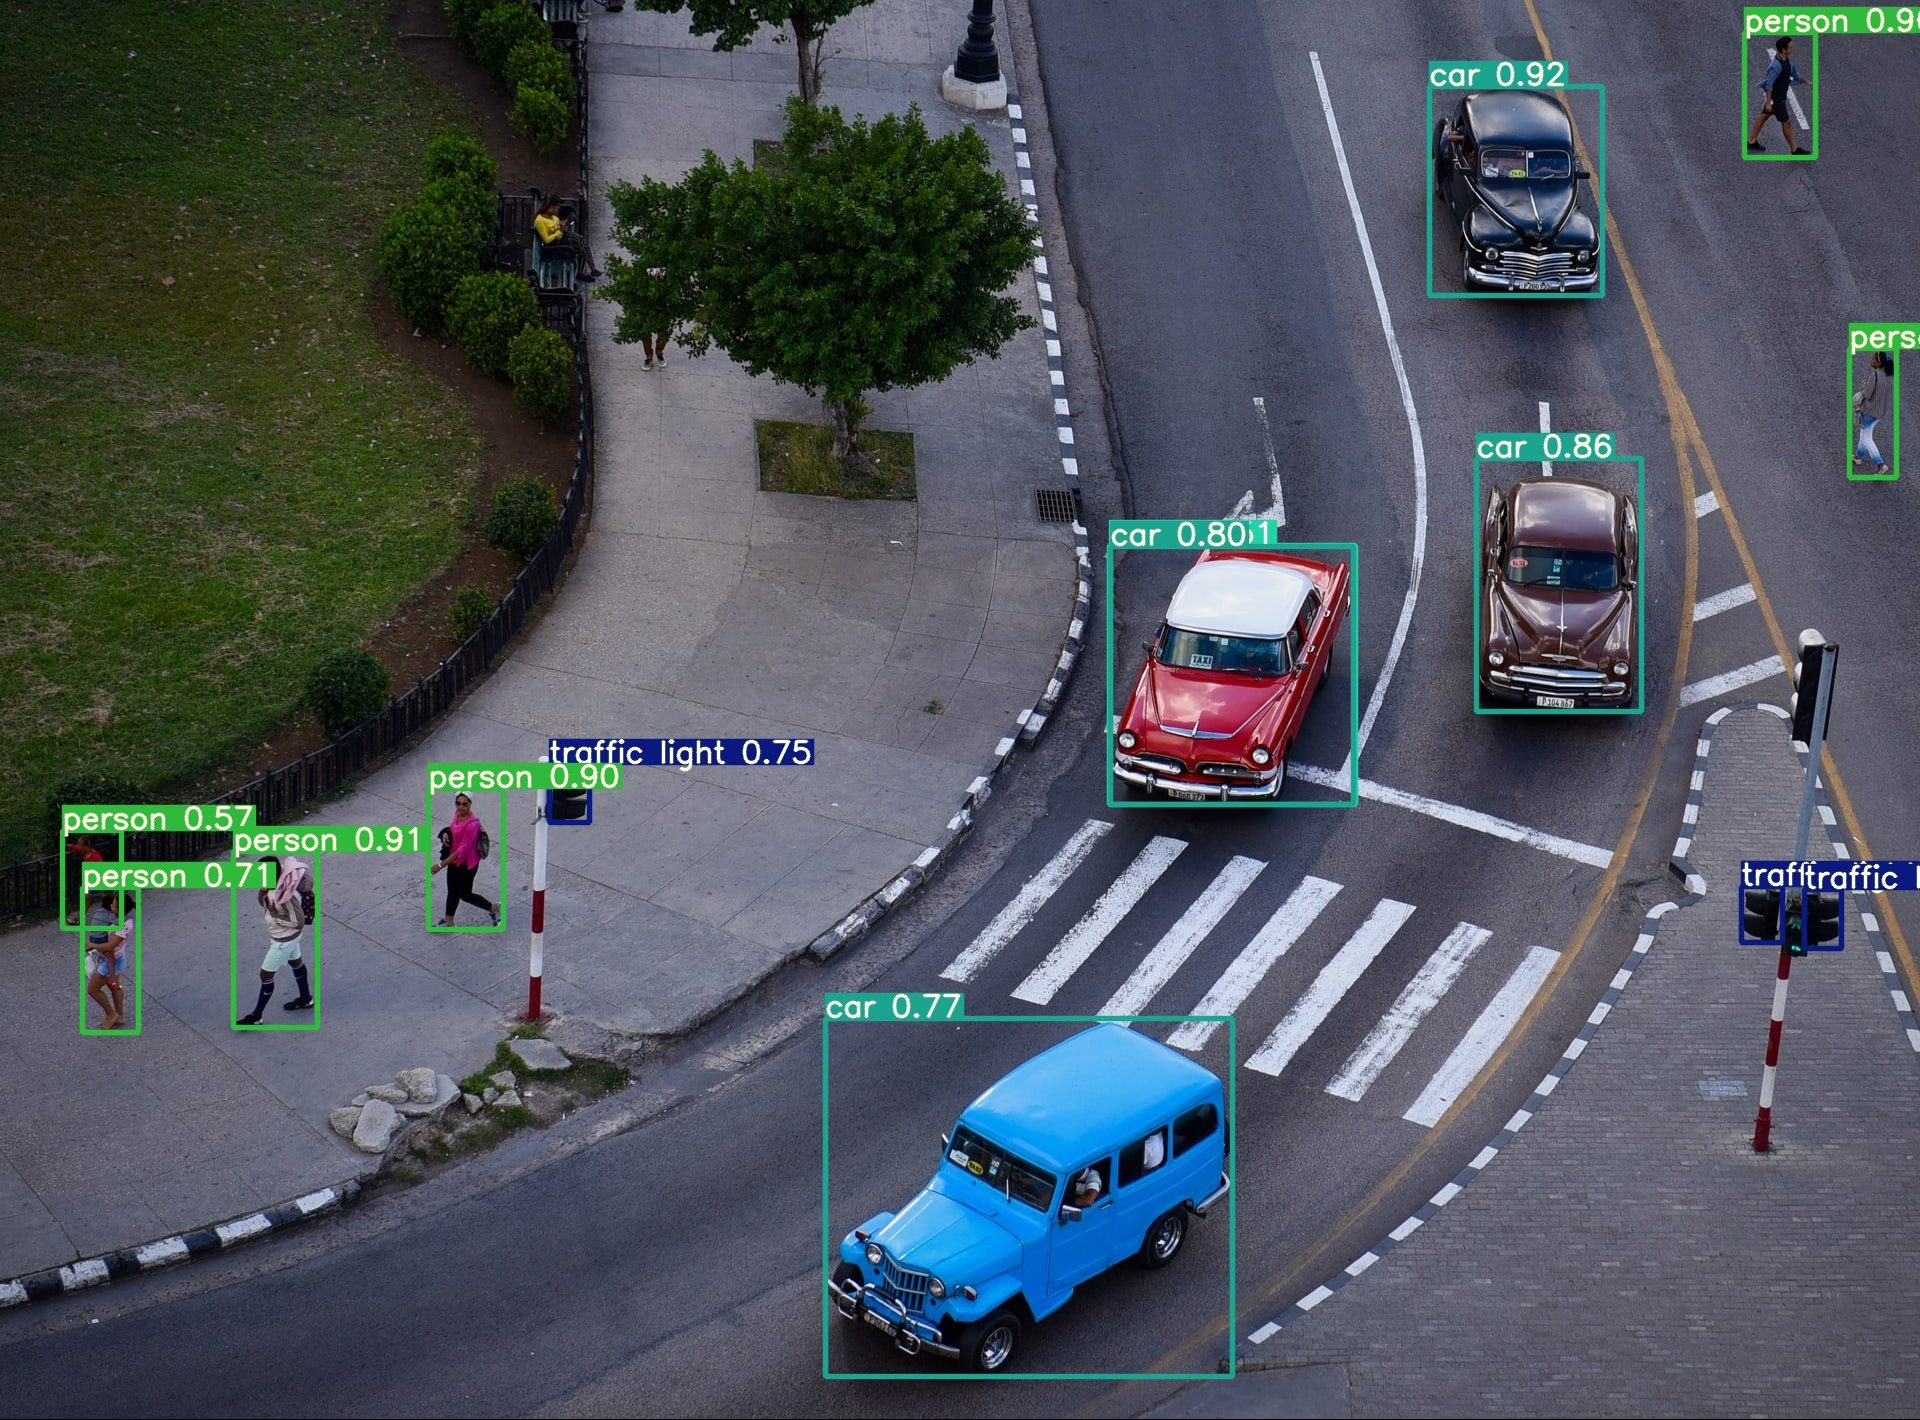
\includegraphics[scale=0.1]{yolo_img.jpg} 
        \end{figure}

        \column{0.5\textwidth}
        \centering
        \begin{figure}
            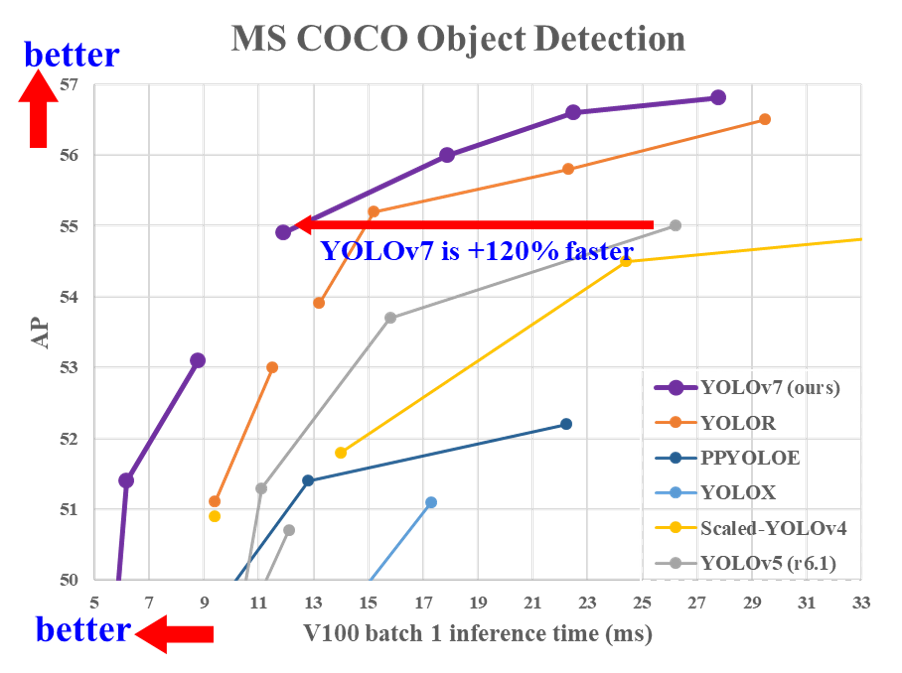
\includegraphics[scale=0.35]{../performance.png}
        \end{figure}
    \end{columns}
\end{frame}

\section{Objektumkövetés}
\begin{frame}{Objektumkövetés}
    \centering
    \begin{figure}
        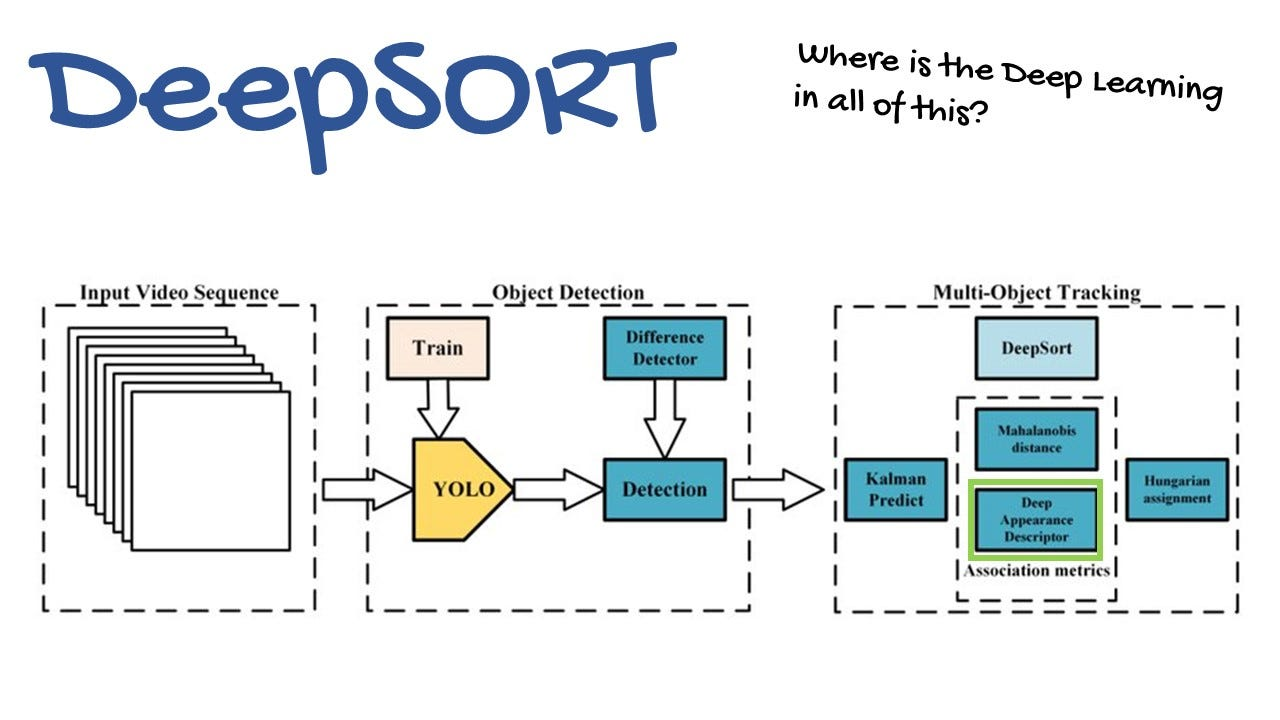
\includegraphics[scale=0.25]{deepsort_flowchart.jpg} 
    \end{figure}
\end{frame}

\section{Machine Learning}
\begin{frame}{Machine Learning}
    \centering
    \begin{figure}
        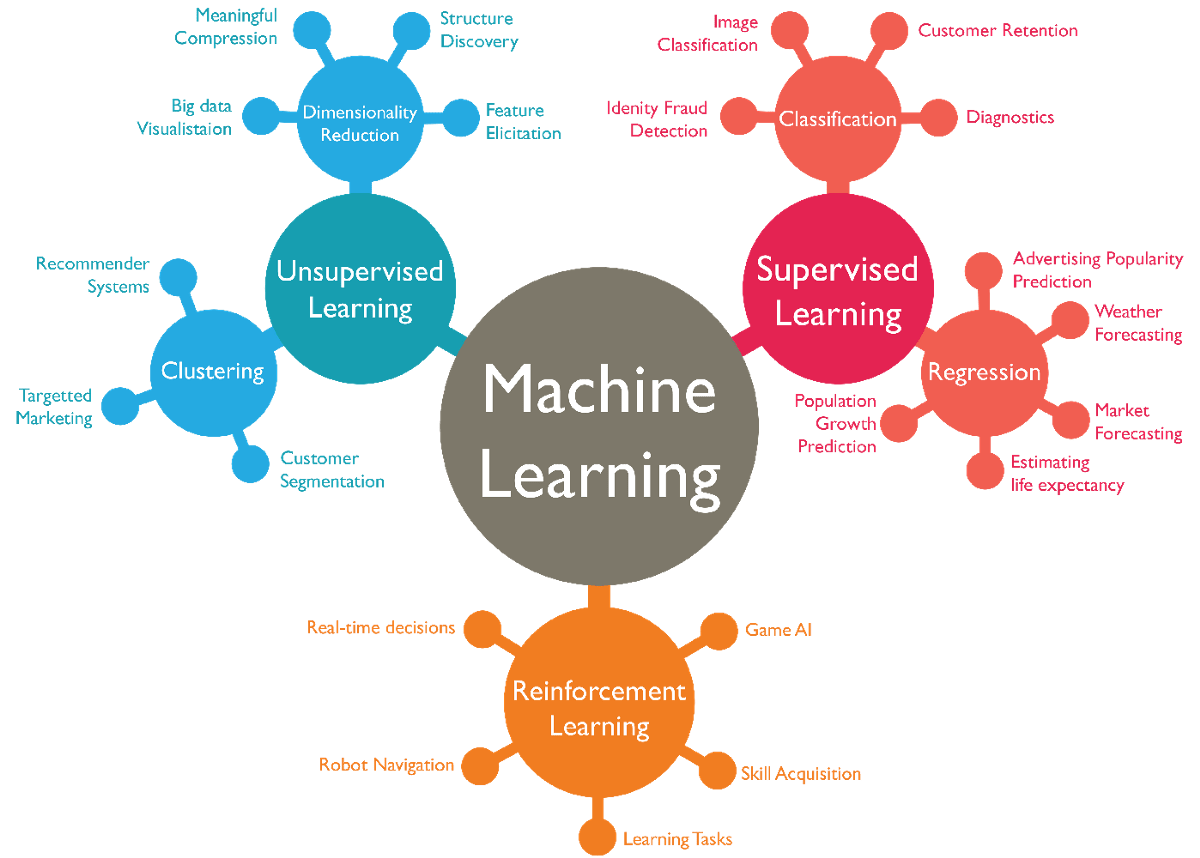
\includegraphics[scale=0.2]{machine_learning.png}    
    \end{figure}
\end{frame}
\subsection{Unsupervised learning}
\begin{frame}{Unsupervised learning}
    \begin{itemize}
        \item Nincsenek előre meghatározott osztályok
        \item Az algoritmus saját maga próbálja csoportokba rendezni a adatokat
    \end{itemize}
    \begin{figure}
        \includegraphics[scale=0.3]{unsupervised_learning.png}
    \end{figure}
\end{frame}
\subsection{Supervised learning}
\begin{frame}{Supervised learning}
    \begin{itemize}
        \item Előre meghatározott osztályok alapján
        \item Az algoritmust tanítani kell példa adatokkal 
        \item Amiket vagy kézzel, vagy klaszterezéssel rendezünk osztályokba
    \end{itemize}
    \begin{figure}
        \includegraphics[scale=0.25]{supervised_learning.jpeg}
    \end{figure}
\end{frame}

\section{Klaszterezés}
\begin{frame}{Klaszterezés}
    \begin{itemize}
        \item Bemeneti adatok: gyűjtött trajektóriák objektumdetektálás és követés segítségével
        \item Feature vektorok: trajektóriák be és kimeneti pontjai
    \end{itemize}
    \begin{figure}
        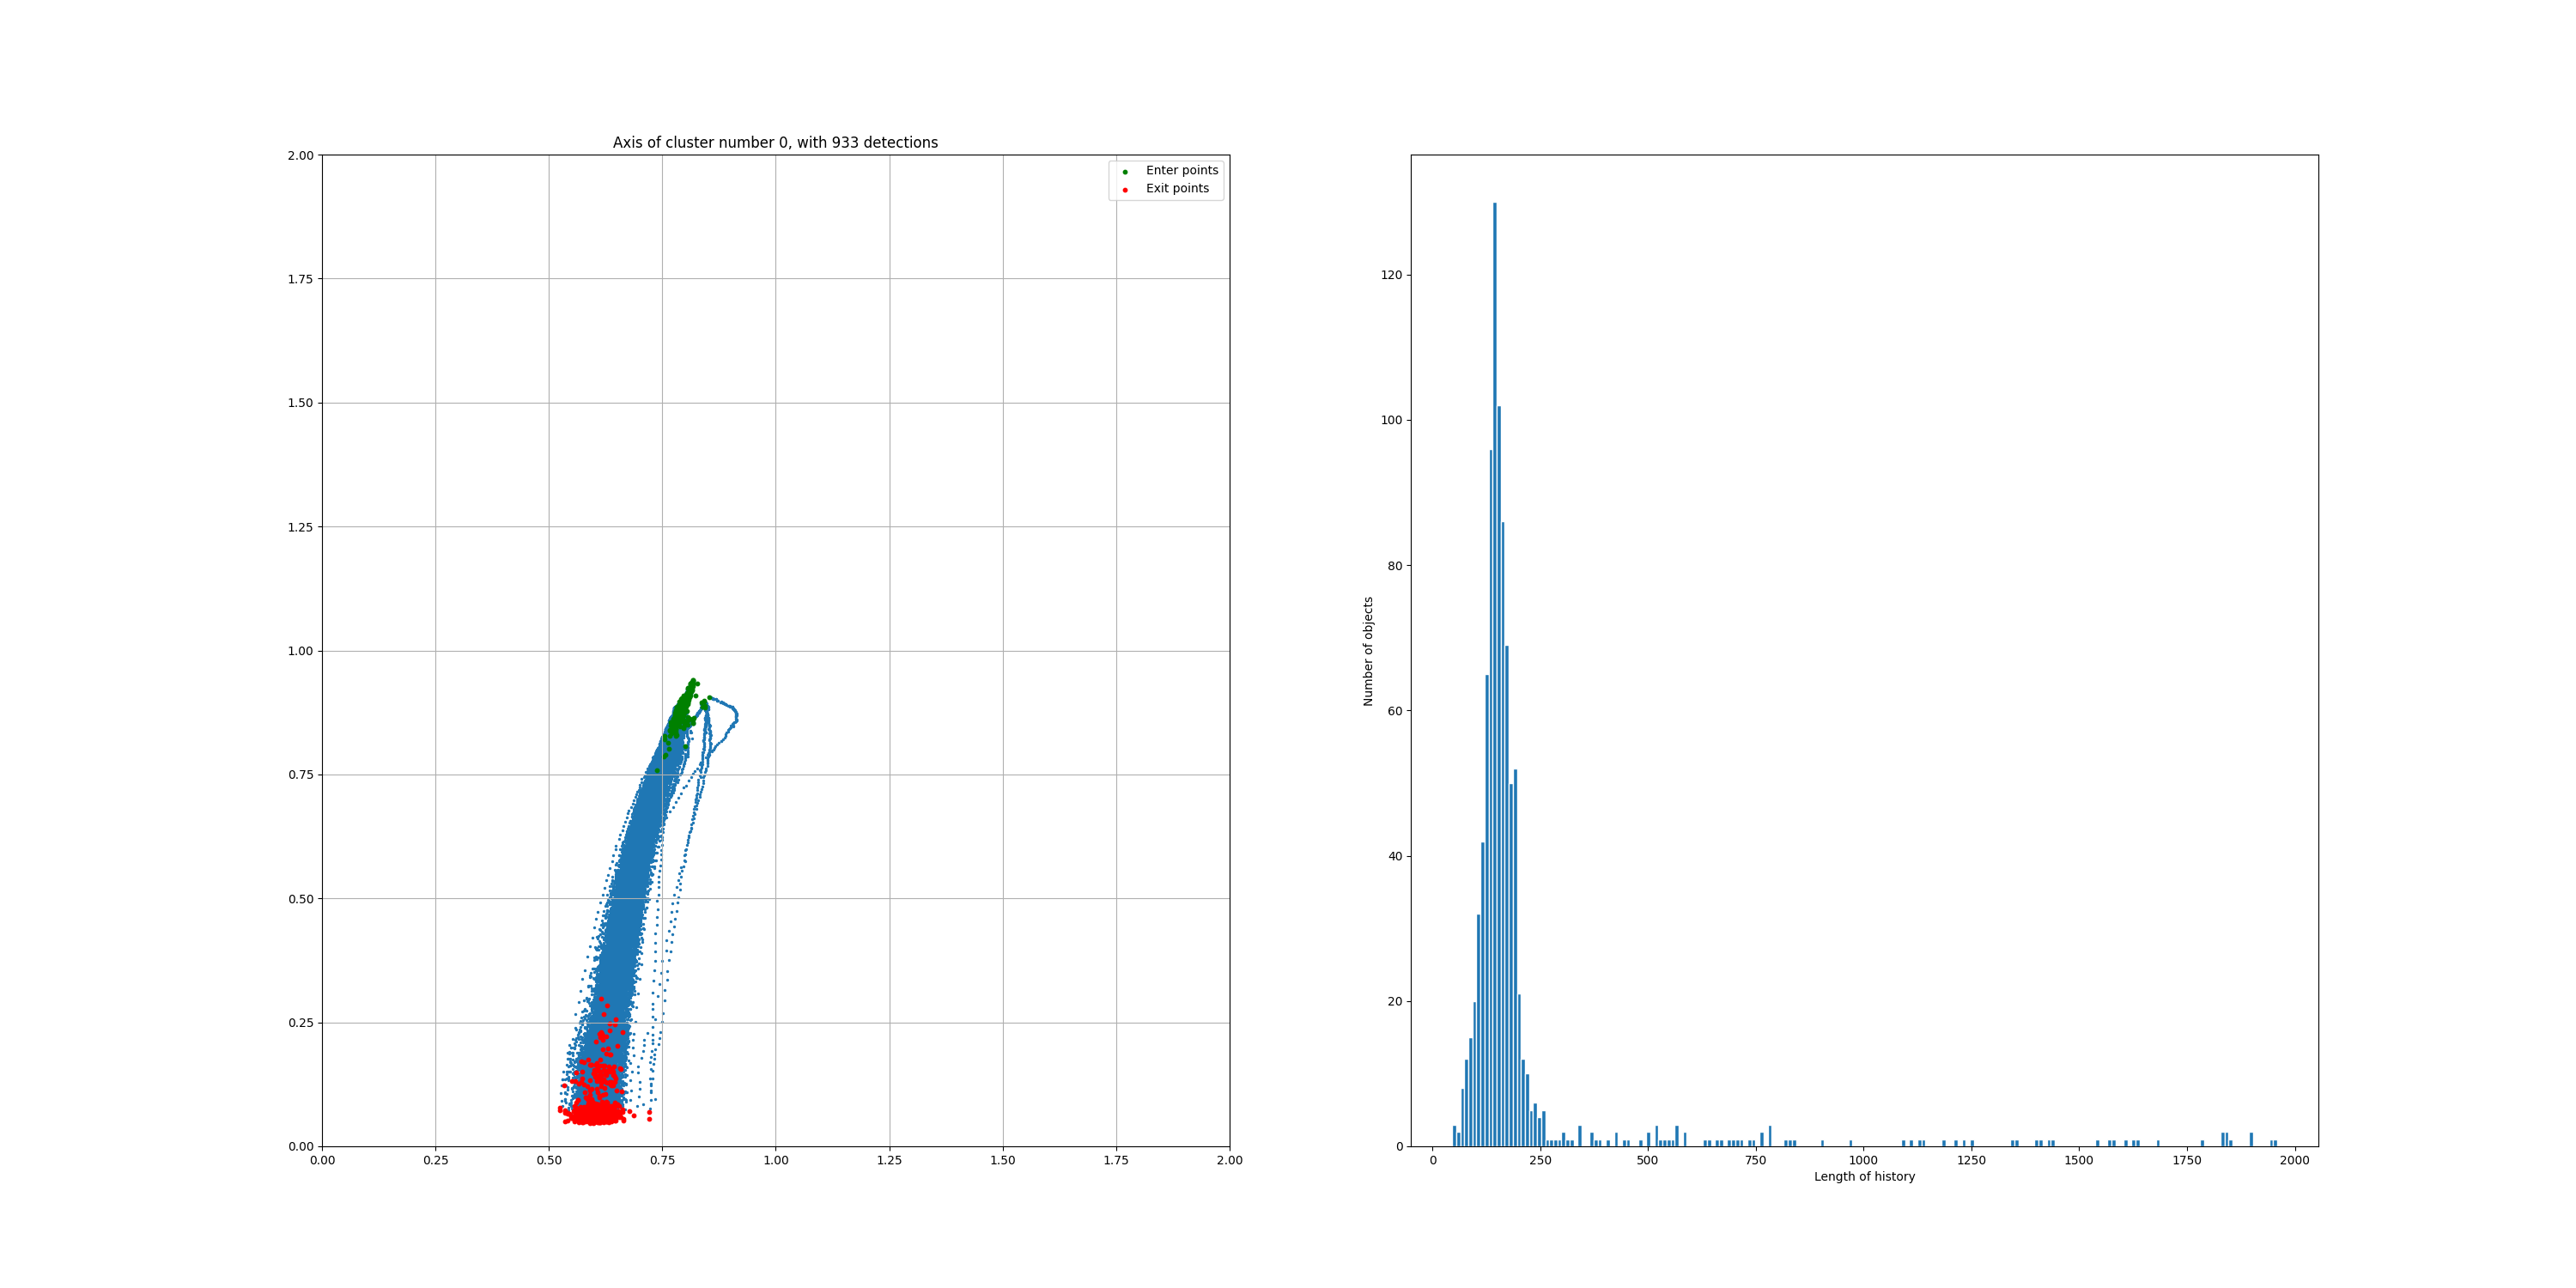
\includegraphics[scale=0.15]{../clustering/n_cluster_0_n_tracks_933.png}
    \end{figure}
\end{frame}

\subsection{Trajektória}
\begin{frame}{Trajektória}
   \begin{figure}
        \includegraphics[scale=0.15]{trajektoriak/car1_1.png}
        \includegraphics[scale=0.15]{trajektoriak/car1_2.png}
        \includegraphics[scale=0.15]{trajektoriak/car1_3.png}
        \includegraphics[scale=0.15]{trajektoriak/car1_4.png}
   \end{figure} 
   \begin{figure}
        \includegraphics[scale=0.2]{trajektoriak/car2_1.png}
        \includegraphics[scale=0.2]{trajektoriak/car2_2.png}
        \includegraphics[scale=0.2]{trajektoriak/car2_3.png}
        \includegraphics[scale=0.2]{trajektoriak/car2_4.png}
   \end{figure} 
\end{frame}

\subsection{Adatok tisztítása}
\begin{frame}{Adatok tisztítása}
    \begin{itemize}
        \item Több különböző zajforrás
        \begin{itemize}
            \item YOLO késői detektálás és követés (a járművet már csak akkor veszi észre amikor bennt van a kereszteződésben)
            \item YOLO fals detektálás (rendőrlámpát vagy táblát autónak néz)
            \item DeepSORT áttapadások (egymáshoz közel elhaladó járművek identitása felcserélődik)
        \end{itemize} 
        \item Megoldások
        \begin{itemize}
            \item Kép relatív széleinek megtalálása min-max kereséssel (az utakat nem biztos, hogy a kép szélétől széléig látjuk, hanem a kép közepétől kezdődve, ezt okozhatja egy nagy épület)
            \item Szűrés trajektóriák kezdő és végpontjainak euklideszi távolsága alapján
            \item Szűrés trajektóriák egymást követő detektálásai közötti távolságokkal
        \end{itemize} 
    \end{itemize}   
\end{frame}

\subsection{Zajos vs Szűrt}
\begin{frame}{Zajos vs Szűrt}
    \begin{figure}
        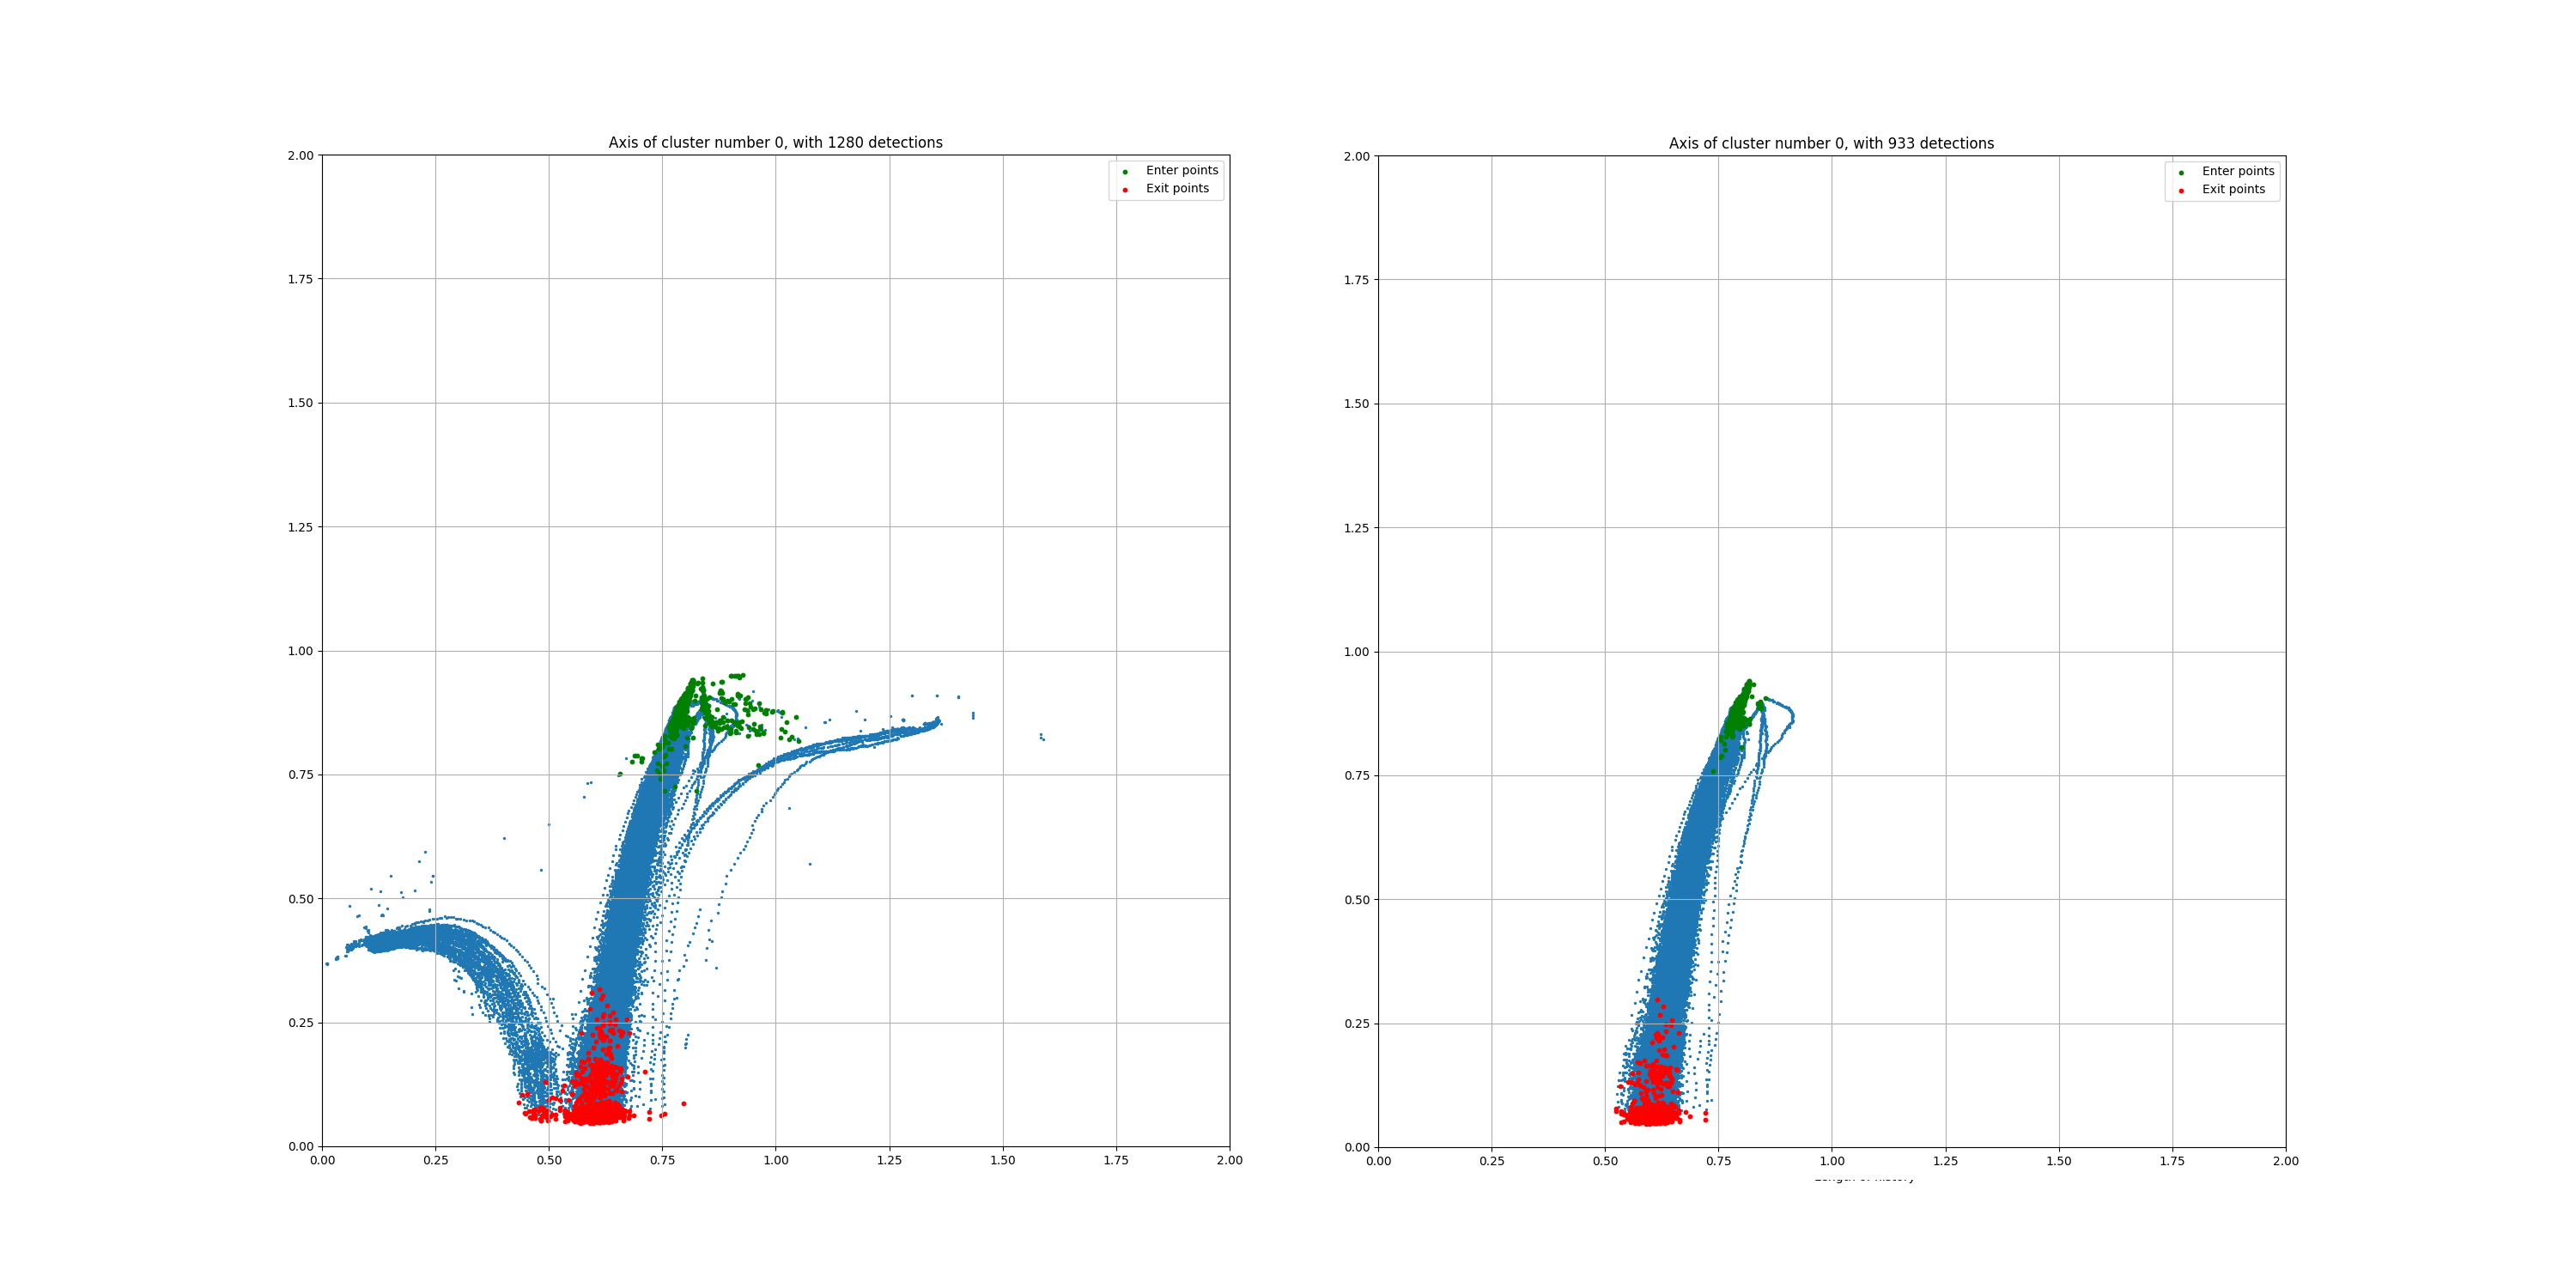
\includegraphics[scale=0.1]{../clustering/n_cluster_0_before_after.png}
        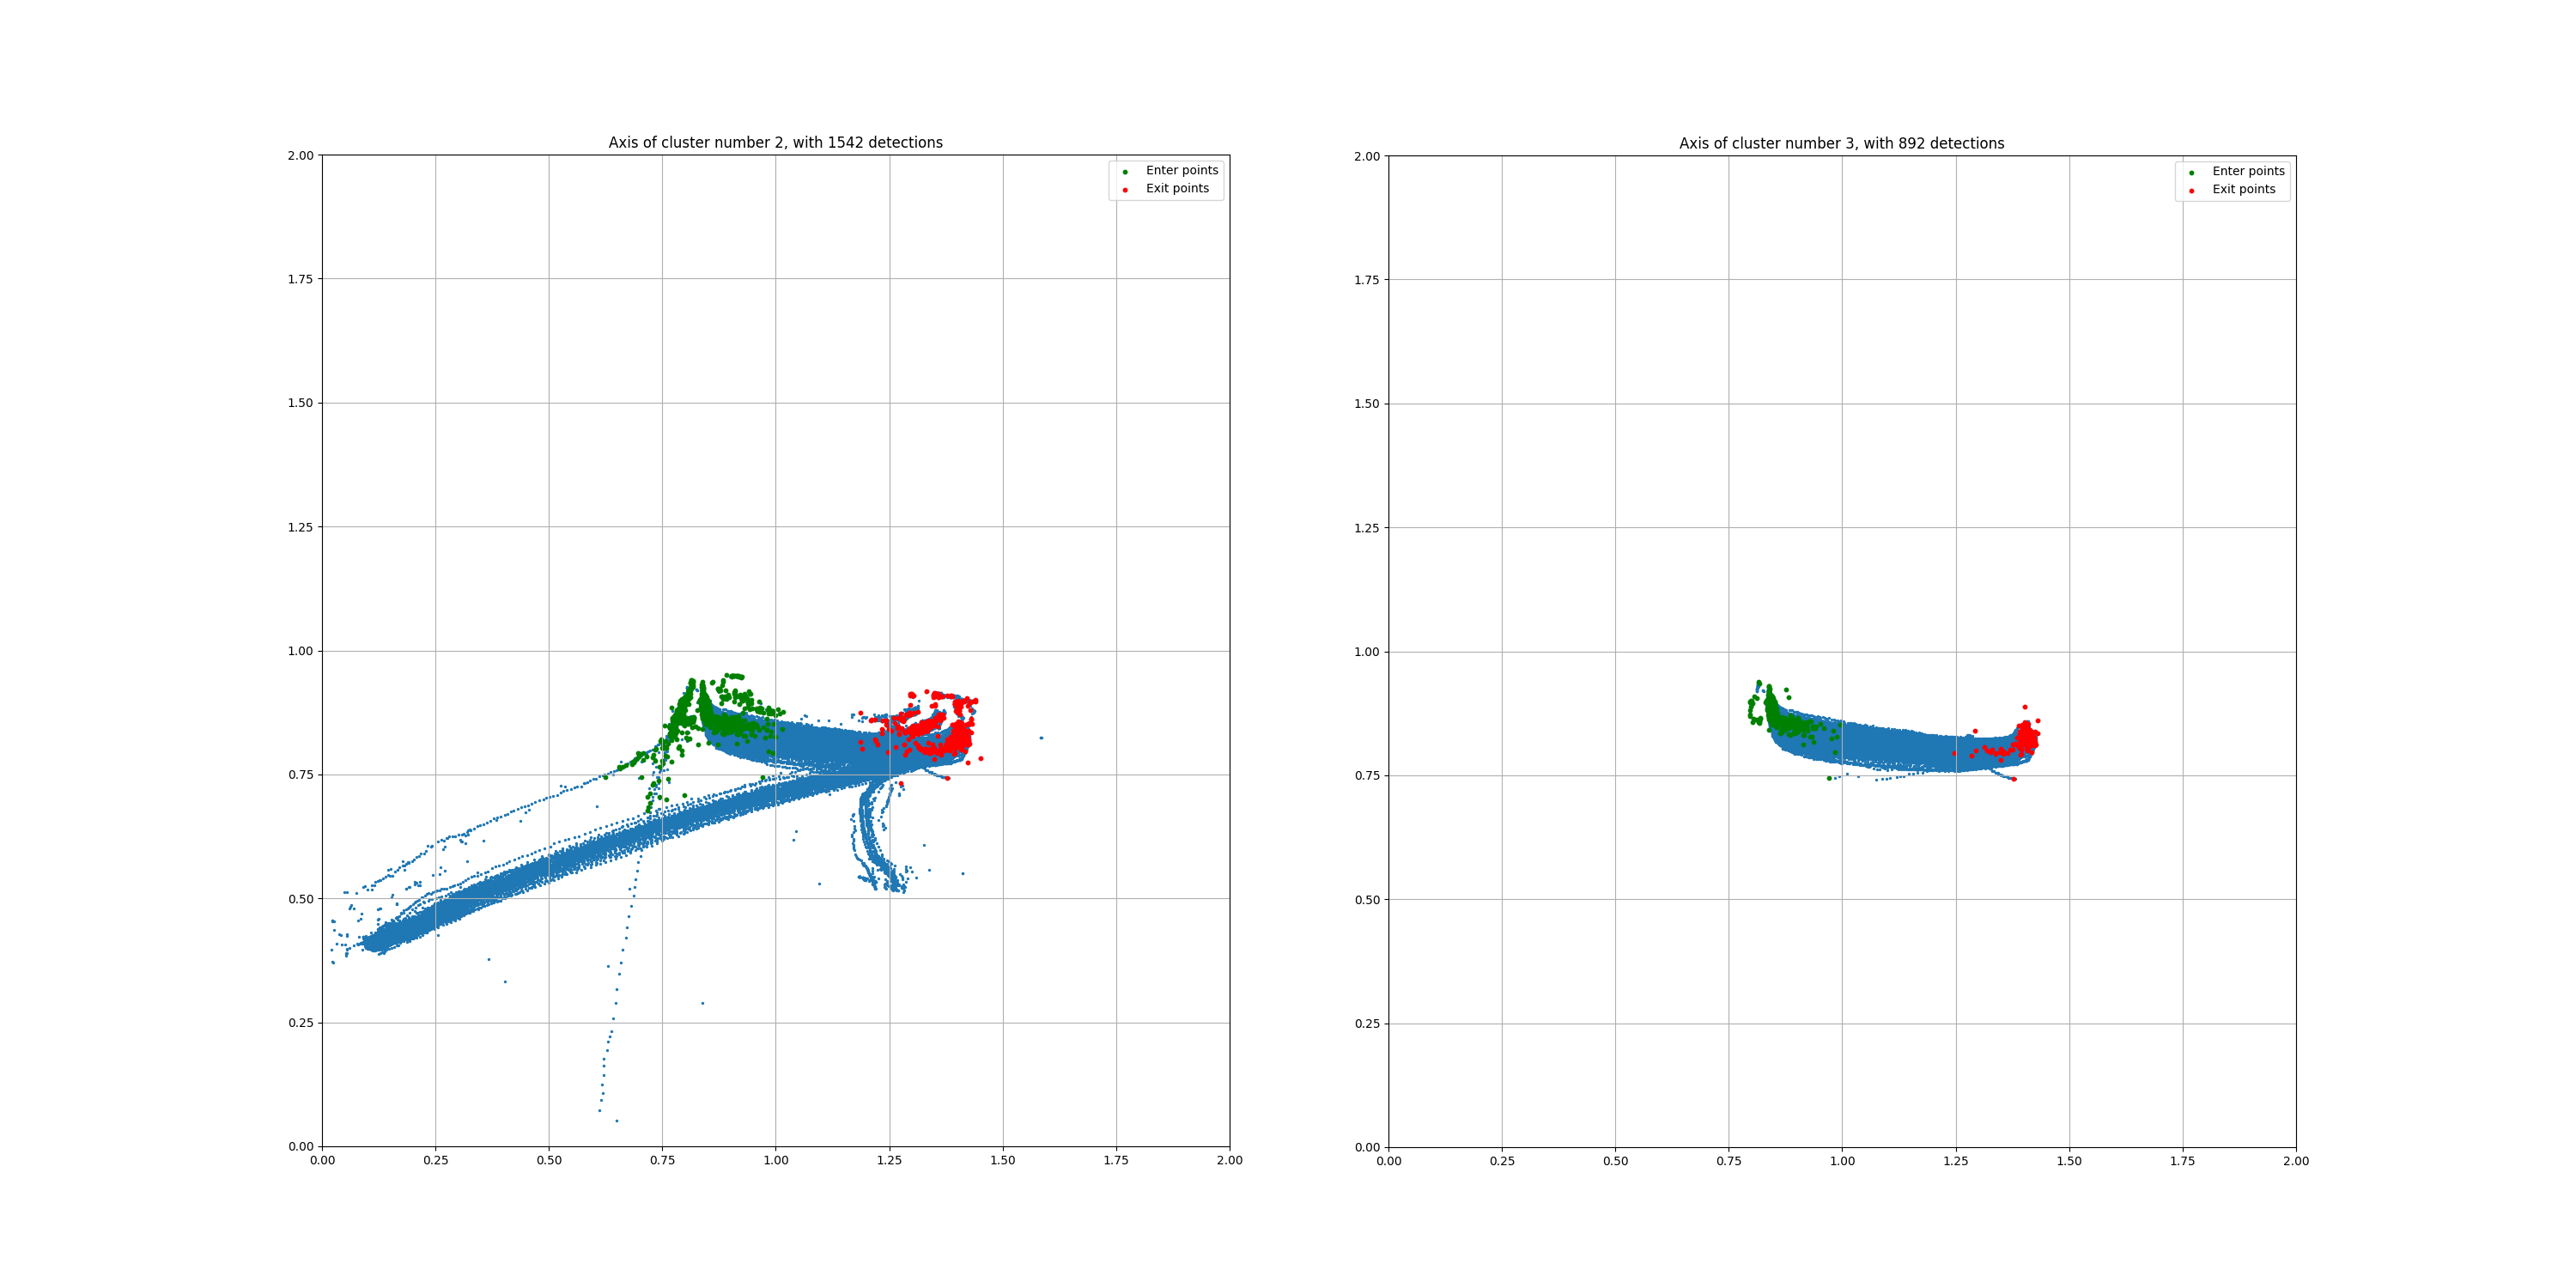
\includegraphics[scale=0.1]{../clustering/n_cluster_2_before_after.png}
    \end{figure}
\end{frame}

\section{Klasszifikáció}
\begin{frame}{Klasszifikáció}

\end{frame}

\section{Alkalmazás}
\begin{frame}{Alkalmazás}
    \centering
    \movie[showcontrols=true]{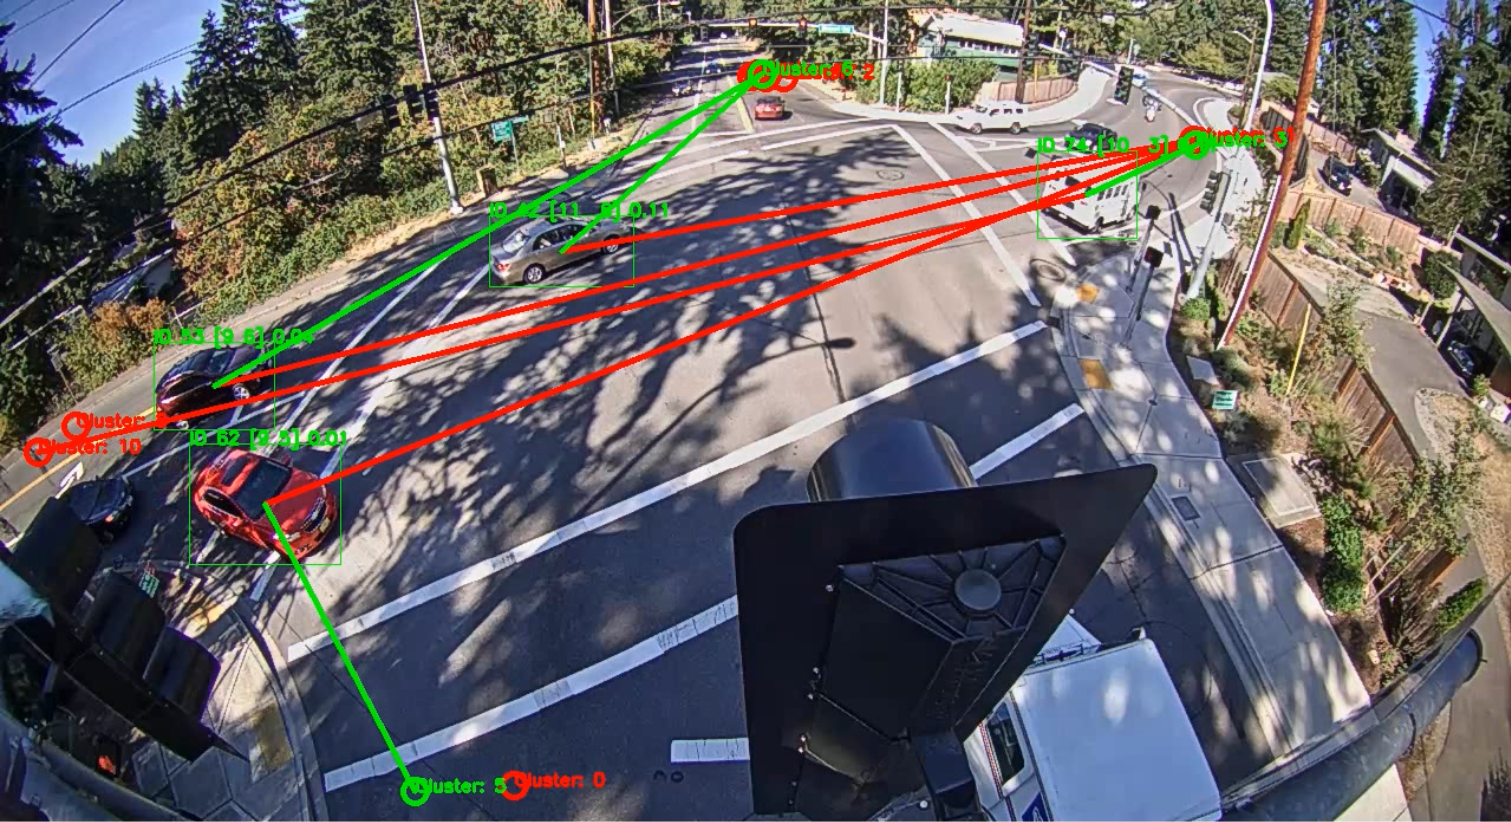
\includegraphics[scale=0.2]{../visualization/bellevue_newport.png}}{./Newport_binary_KNN_n_neighbors_15_stride-15_v7.mp4}
\end{frame}



\end{document}